\renewcommand{\thechapter}{\roman{chapter}}
\setcounter{chapter}{1}
\setcounter{figure}{0}

\unchapter{Introduction}
\label{chap:introduction}
La peau est un des organes les plus important du corps humain et recouvre l'ensemble de celui-ci. Ses lésions sont nombreuses~: des plus anodines communément appelées lésions bénignes, aux plus graves d'entre elles regroupées sous le terme de lésions malignes. Ces lésions malignes sont d'origine cancéreuse et engendrent des répercussions dramatiques lorsque qu'elles ne sont pas traitées à temps.\par

Ainsi, ces lésions malignes sont issues d’une division ou d’une mutation anormale de cellules de la peau. Leur cancérogénèse est le fait d'altérations du matériel génétique congénital sous l'effet d'agents extérieurs chimiques, tel que le tabac ou les médicaments, mais aussi viraux. Néanmoins, ces altérations ont le plus souvent pour origine l'action de radiations ionisantes. Ces radiations ionisantes impliquées dans la survenue des cancers cutanés sont essentiellement d'origine naturelle (soleil) mais peuvent être aussi d'origine artificielle~: lors de loisirs (cabines de bronzage) ou lors de thérapies (radiothérapie).\par

Afin de limiter l’incidence de ces tumeurs, de nombreuses campagnes de prévention sont menées au sein des pays les plus touchés, intégrant une dimension de sensibilisation et des actions de prévention dans le but d’augmenter le confort de vie futur des individus et de limiter les dépenses de santé en prévenant l'apparition des tumeurs malignes. Ces campagnes de sensibilisation à la prévention, bien que souvent sous des formes plus traditionnelles tel que des prospectus ou messages publicitaires, peuvent prendre diverses formes afin de toucher au mieux leurs cibles. A titre d’exemple, 
peuvent être cités la mise en place de formations de prévention dès le plus jeune âge au sein des structures scolaires aux États-Unis, ou la multiplication des supports de communication avec, par exemple, l’utilisation de sachets de sucre au Portugal~\cite{Correia2017,Guy2016}.\par 

Néanmoins, les mesures de sensibilisation tendent aujourd’hui à dépasser la prévention et s'orientent vers la sensibilisation des individus à l'auto-surveillance. Certains articles montrent l’importance d’une auto-surveillance régulière des individus par des gestes à la portée de tous, permettant une prise en charge des pathologies dans un meilleur délai. Dans ce même objectif, l’accroissement du nombre de campagnes de dépistage mises en place par les gouvernements peut-être mentionné~\cite{Friedman1985}. Ces diverses actions sont particulièrement efficaces pour permettre la détection de mélanomes à des stades moins avancés, et donc plus susceptibles d'être correctement pris en charges et traités.\par

Malgré ces nombreuses démarches, le taux d’apparition de ces cancers ne cesse d’augmenter dans le monde. Ces dernières années, l'\gls{who} dénombre entre 2 et 3 millions de cancers de la peau par an, dont environ 360 000 sont des mélanomes. Ces chiffres sont corroborées par ceux d'études épidémiologiques dont les recensements ont été réalisés en 2015~\cite{Vos2016}, dont la \Cref{tab:introduction_cancer_incidence} reprend les diverses données. Ainsi, certaines régions du globe comme l'Australasia ou encore l'Amérique du Nord sont particulièrement touchées par cette recrudescence des maladies de la peau avec de fortes incidences~\cite{Karimkhani2017}. De même, au niveau des populations touchées, le facteur d'âge semble être un critère de risque important~\cite{Karimkhani2017}.\par 

\begin{table}[H]
    \centering
    \begin{tabular}{lll}
    \toprule
    \textbf{Emplacement ou dénomination}& \textbf{Incidence}& \textbf{Décès}\\ \midrule
    Tous                                & 17481             & 8713          \\  
    Lèvre et cavité buccale             & 410               & 146           \\  
    Nasopharynx                         & 123               & 63            \\  
    Autre pharynx                       & 161               & 64            \\  
    Œsophage                            & 1313              & 891           \\  
    Côlon et rectum                     & 1653              & 832           \\
    Vésicule et voies biliaires         & 188               & 140           \\
    Pancréas                            & 426               & 412           \\
    Larynx                              & 238               & 106           \\
    Trachée, des bronches et du poumon  & 2019              & 1722          \\
    Sein                                & 2422              & 534           \\
    Col utérin                          & 526               & 239           \\
    Utérus                              & 455               & 90            \\
    Ovaires                             & 251               & 161           \\
    Prostate                            & 1618              & 366           \\
    Testicules                          & 72                & 9             \\
    Rein                                & 425               & 137           \\
    Vessie                              & 541               & 188           \\
    Système nerveux                     & 321               & 229           \\
    Thyroïde                            & 334               & 32            \\
    \textbf{Mélanome}                   & \textbf{352}      & \textbf{60}   \\
    Mésothéliome                        & 37                & 32            \\
    Lymphome de Hodgkin                 & 78                & 24            \\
    Lymphome non hodgkinien             & 666               & 231           \\
    Mélyome multiple                    & 154               & 101           \\
    Leucémie                            & 606               & 353           \\
    Leucémie lymphoïde aiguë            & 161               & 110           \\
    Leucémie lymphoïde chronique        & 191               & 61            \\
    Leucémie myéloïde aiguë             & 190               & 147           \\
    Leucémie myéloïde chronique         & 64                & 35            \\
    Autres néoplasmes                   & 756               & 372           \\ \bottomrule
    \end{tabular}   
    \caption{Statistiques mondiales d’incidence et mortalité des cancers par emplacements~\cite{Karimkhani2017}. Les chiffres indiqués dans le tableau (incidence et décès) sont exprimés en milliers.}
    \label{tab:introduction_cancer_incidence}
\end{table}\par

Pour la France, ce n’est pas moins de 80 000 nouveaux cas de cancers de la peau estimés en 2015, dont 70\% d'entre eux sont des carcinomes basocellulaires~\textsuperscript{\ref{footnote:number_dermatologists}}, soit la 6ème cause de cancer en France. Pour leur part, les mélanomes sont eux estimés à 14 300 cas par an dont 1 773 engendrent un décès~\cite{Thuret2012}. Une détection précoce de ces tumeurs est donc nécessaire en termes de santé publique mais aussi économique, bien qu'il soit difficile d'obtenir des chiffres sur les coûts engendrés par ces pathologies pour la France. Néanmoins à titre d'exemple, les soins générés par les pathologies de la peau se chiffrent annuellement à 8 milliards de dollars aux États-Unis~\cite{Farberg2017a}.\par

\addtocounter{footnote}{1}
\footnotetext[\thefootnote]{Source~: Chiffres issus du site de la \href{https://www.frm.org/}{Fondation pour la Recherche Médicale}. \label{footnote:number_skin_france}}

Le sujet de ce manuscrit « \titleref » s’inscrit dans cette thématique et tente d’apporter des méthodes pour permettre une aide au diagnostic des praticiens en dermatologie dans un contexte clinique de plus en plus contraignant. En effet, cette thèse répond en premier lieu à un besoin sociétal, si l'on considère la baisse constante du nombre de dermatologues en France depuis 2010, visible sur la \Cref{fig:number_dermatologists}. L'aboutissement de ce travail est donc d'augmenter la capacité de diagnostic tant de l'expert que du non expert, en optimisant les examens cliniques nécessaires et en réduisant le temps passé à la réalisation des divers examens.\par

\begin{figure}[H]
    \centering
    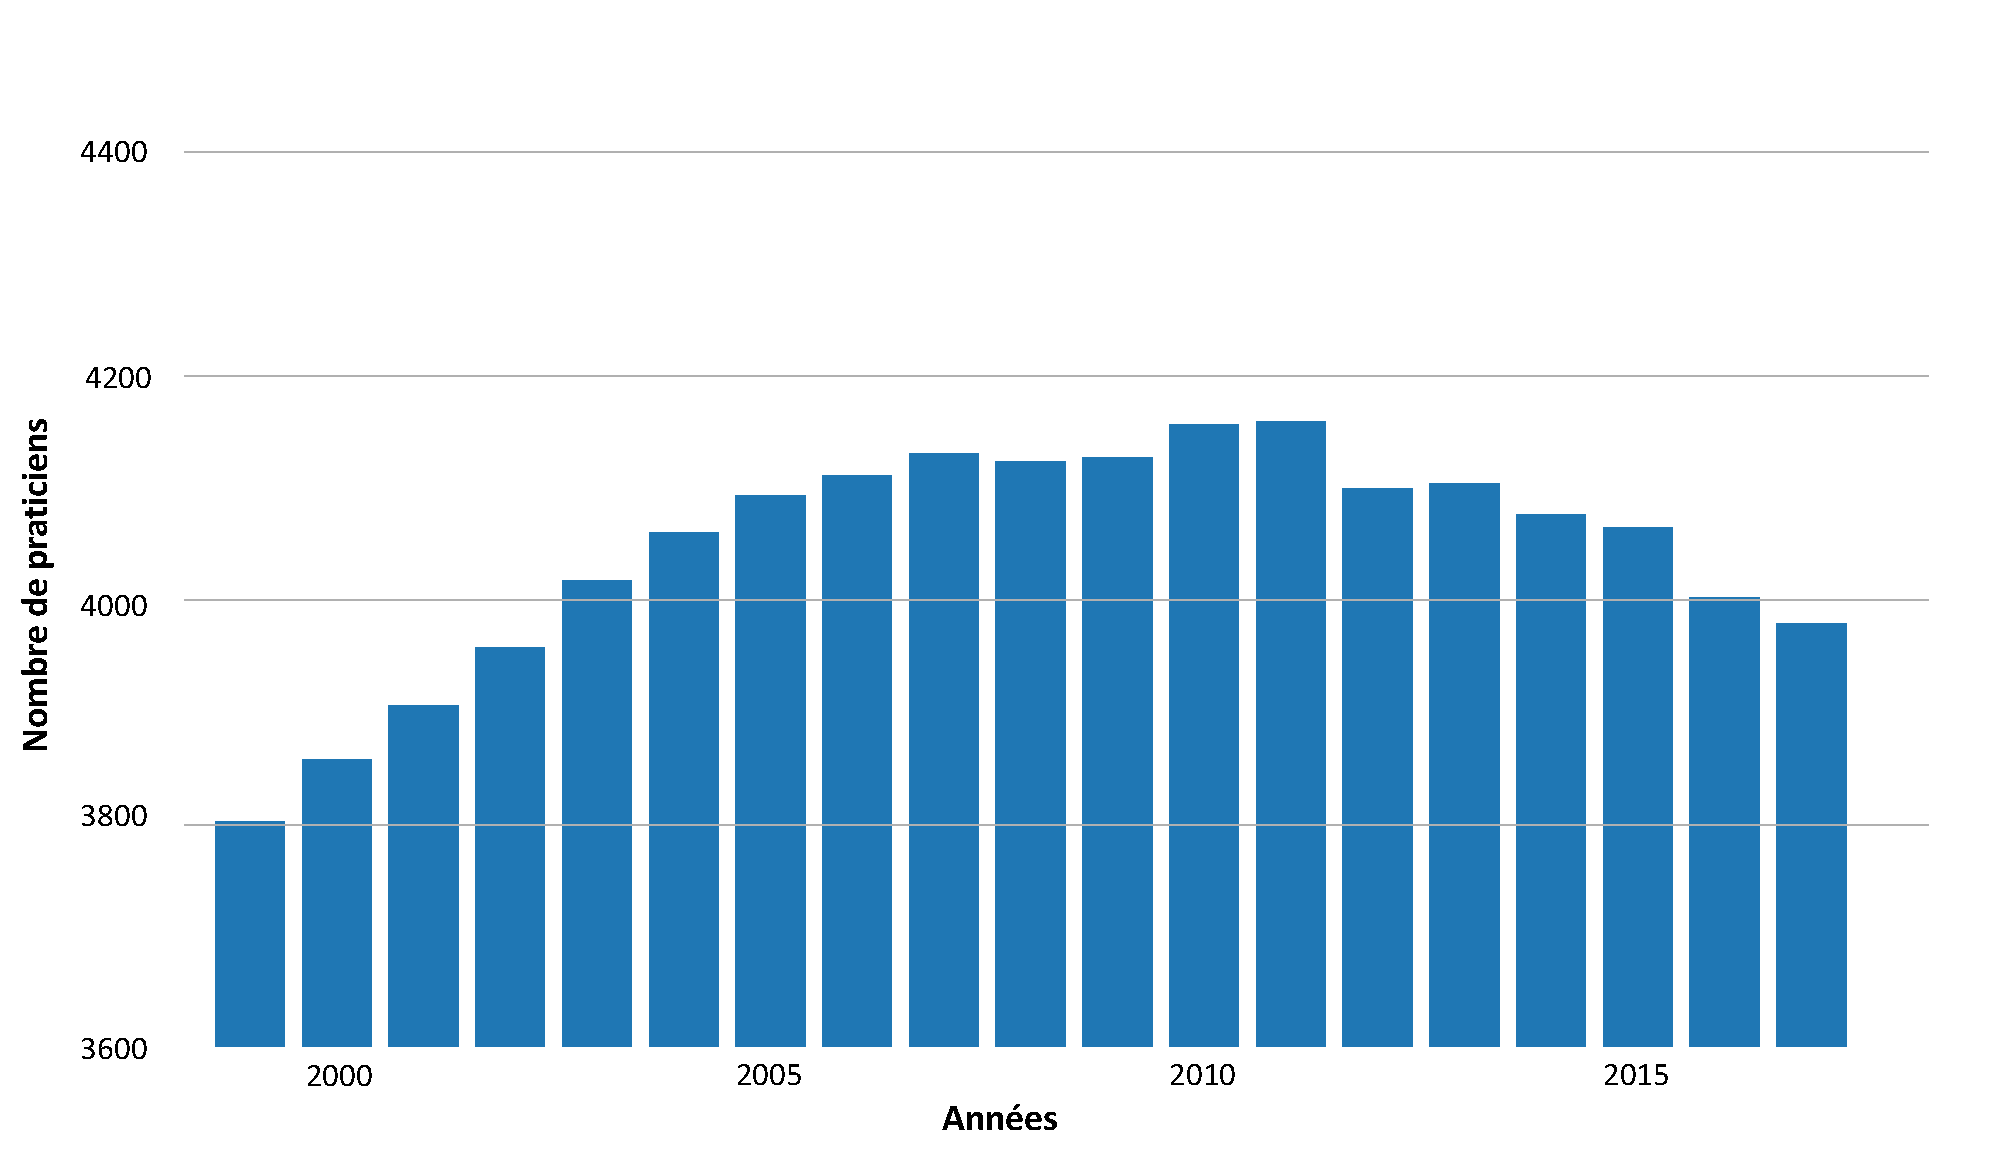
\includegraphics[width=\linewidth]{contents/i_introduction/resources/evolution_dermatologists.pdf}
    \caption{Graphique représentant l'évolution du nombre de dermatologues en France entre les années 1999 et 2017 \textsuperscript{\ref{footnote:number_dermatologists}}.}
    \label{fig:number_dermatologists}
\end{figure}\par
\addtocounter{footnote}{1}
\footnotetext[\thefootnote]{Source image~: Graphique généré à partir de données en provenance du site du \href{http://www.data.drees.sante.gouv.fr/}{gouvernement} sur la santé. \label{footnote:number_dermatologists}}

Outre cette réponse à un besoin sociétal, cette thématique ne demeure pas moins intéressante d’un point de vue scientifique. L’intérêt scientifique pour l'utilisation des outils d'aide au diagnostic en pratique dermatologique se traduit notamment par une forte tendance sur le sujet comme le démontre la \Cref{fig:evolution_publications}. Cette tendance est régie par plusieurs facteurs~:
\begin{itemize}
    \item Le \textbf{besoin sociétal} de la thématique déjà évoqué lors du précédent paragraphe et \textbf{l'intérêt des industriels} de proposer des biens et des services permettant une meilleur efficience des professionnels du domaine.
    \item Le \textbf{phénomène de l'apprentissage automatique} ou \textit{machine learning} qui résulte d'un engouement stimulé par des avancées constantes et soutenues du domaine mais aussi de la démocratisation des méthodes qui en sont issues. 
    \item Le \textbf{défi scientifique} apporté par cette thématique de dermatologie, qui regroupe d'une part les données de travail (les appareils d'acquisition, les conditions d'acquisition, \ldots) et d'autre part l'information à extraire des données. Ces divers éléments sont approfondis tout au long de ce manuscrit.
\end{itemize}\par
\clearpage

Ce travail s'inscrit dans une démarche d'aide au diagnostic des lésions de la peau et particulièrement des pathologies de \gls{lm} et \gls{lmm}. De nombreux travaux se sont portés sur l'aide à la détection par ordinateur de lésions de la peau à partir d'une modalité unique d'imagerie. Néanmoins, peu d'entre eux s'intéressent à une démarche multimodale de cette thématique, dû à la complexité que gènère une telle étude ou bien par manque ou insuffisance de données à leur disposition.\par

\begin{figure}[H]
    \centering
    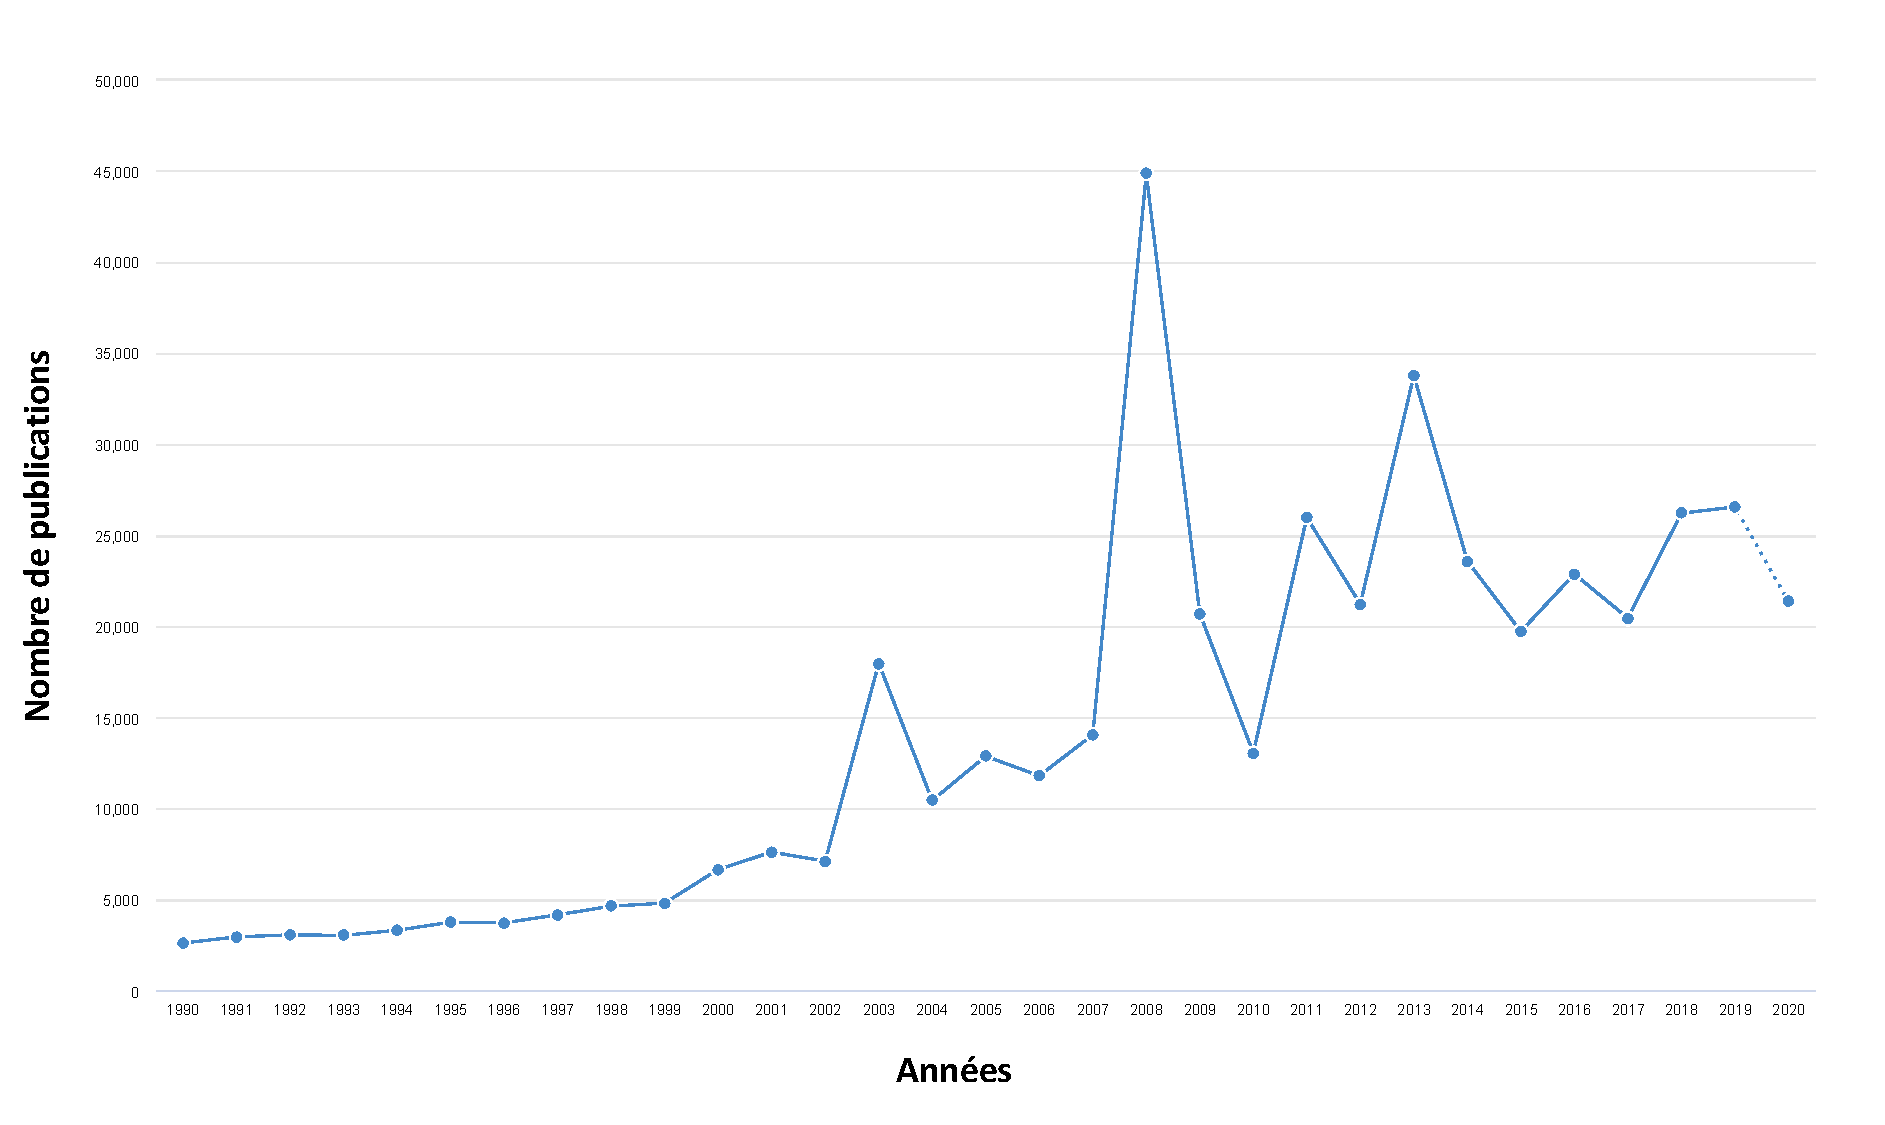
\includegraphics[width=\linewidth]{contents/i_introduction/resources/evolution_publications.pdf}
    \caption{Graphique représentant l'évolution du nombre de publications recensées par le moteur \href{https://scholar.google.fr/}{Google Scholar}~\textsuperscript{\ref{footnote:evolution_publications}} autour des termes de « skin computer diagnosis » lors de ces trente dernières années.}
    \label{fig:evolution_publications}
\end{figure}\par
\addtocounter{footnote}{1}
\footnotetext[\thefootnote]{Source image~: Graphique généré à partir du site \href{https://www.dimensions.ai/}{Dimensions.}  \label{footnote:evolution_publications}}

La matière première mise à notre disposition permet une orientation de ces travaux dans le sens de la multimodalité. En effet, l'une des problématiques majeures aujourd'hui en dermatologie est ce que les médecins qualifient de zone d'indécision, également appelée \textit{zone grise}. Il s'agit d'une catégorie de cas cliniques pour lesquels le médecin n'a pas à un instant $t$ suffisamment d'informations ou de connaissances pour prendre une décision. Ces cas nécessitent souvent une prise en charge plus importante, avec l'aide d'autres spécialistes ou encore avec notamment de nouveaux examens plus spécifiques.\par

La finalité de ce travail est de proposer diverses méthodes et outils permettant une aide à la décision dans la gestion de cette zone grise, et ainsi améliorer la prise en charge clinique en service de dermatologie. A l'instar des travaux existants, cette gestion de la zone grise passe d'une part par l'implémentation de méthodes propres à certaines des modalités de ce travail et d'autre part par la mise en place d'un schéma multimodal. Ainsi, un schéma macroscopique de cet objectif sur la \Cref{fig:scheme_reduce_indecision}.\par
\clearpage

Dans ce schéma idéal représenté sur la \Cref{fig:scheme_reduce_indecision}, les patients jugés avec une certaine certitude comme \textbf{bénins} ou \textbf{malins}, seront exclus des procédures suivantes. Seuls les patients encore présents dans cette \textit{zone grise} sont pris en charge pour des examens supplémentaires, pour lesquels le processus sont réitérés.\par 

\begin{figure}[H]
    \centering
    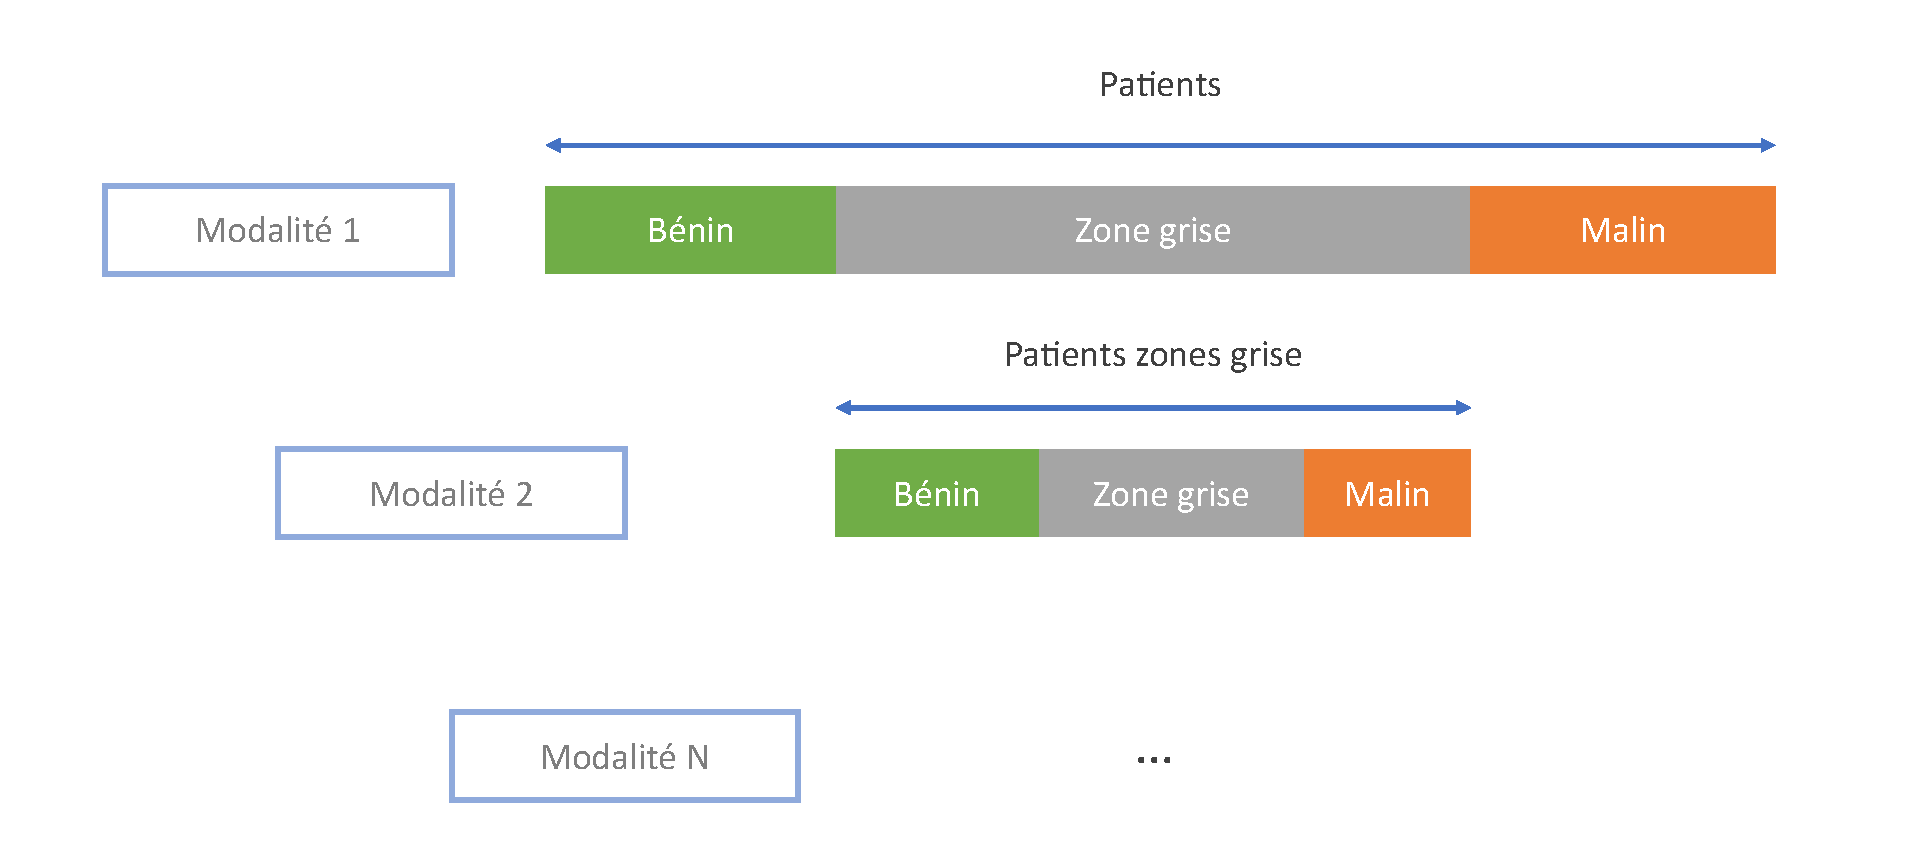
\includegraphics[width=\linewidth]{contents/i_introduction/resources/scheme_reduce_indecision.pdf}
    \caption{Représentation du processus de réduction de l'indécision du médecin ou \textit{zone grise}. L'objectif de ce travail consiste à réduire cette indécision des divers cas d'études en notre possession, par l'ajout de modalités d'imagerie en s'inspirant du processus cognitif des dermatologues.}
    \label{fig:scheme_reduce_indecision}
\end{figure}\par

A cette fin, ce travail mobilise des connaissances en provenance de divers champs d'applications propres~:
\begin{inlinerate}
    \item à la peau d'un point de vue médical, 
    \item aux modalités permettant l'observation des tissus,
    \item et à l'intelligence artificielle.
\end{inlinerate} Cette complémentarité est représentée sous forme de schéma sur la \Cref{fig:scheme_our_work}.\par

\begin{figure}[H]
    \centering
    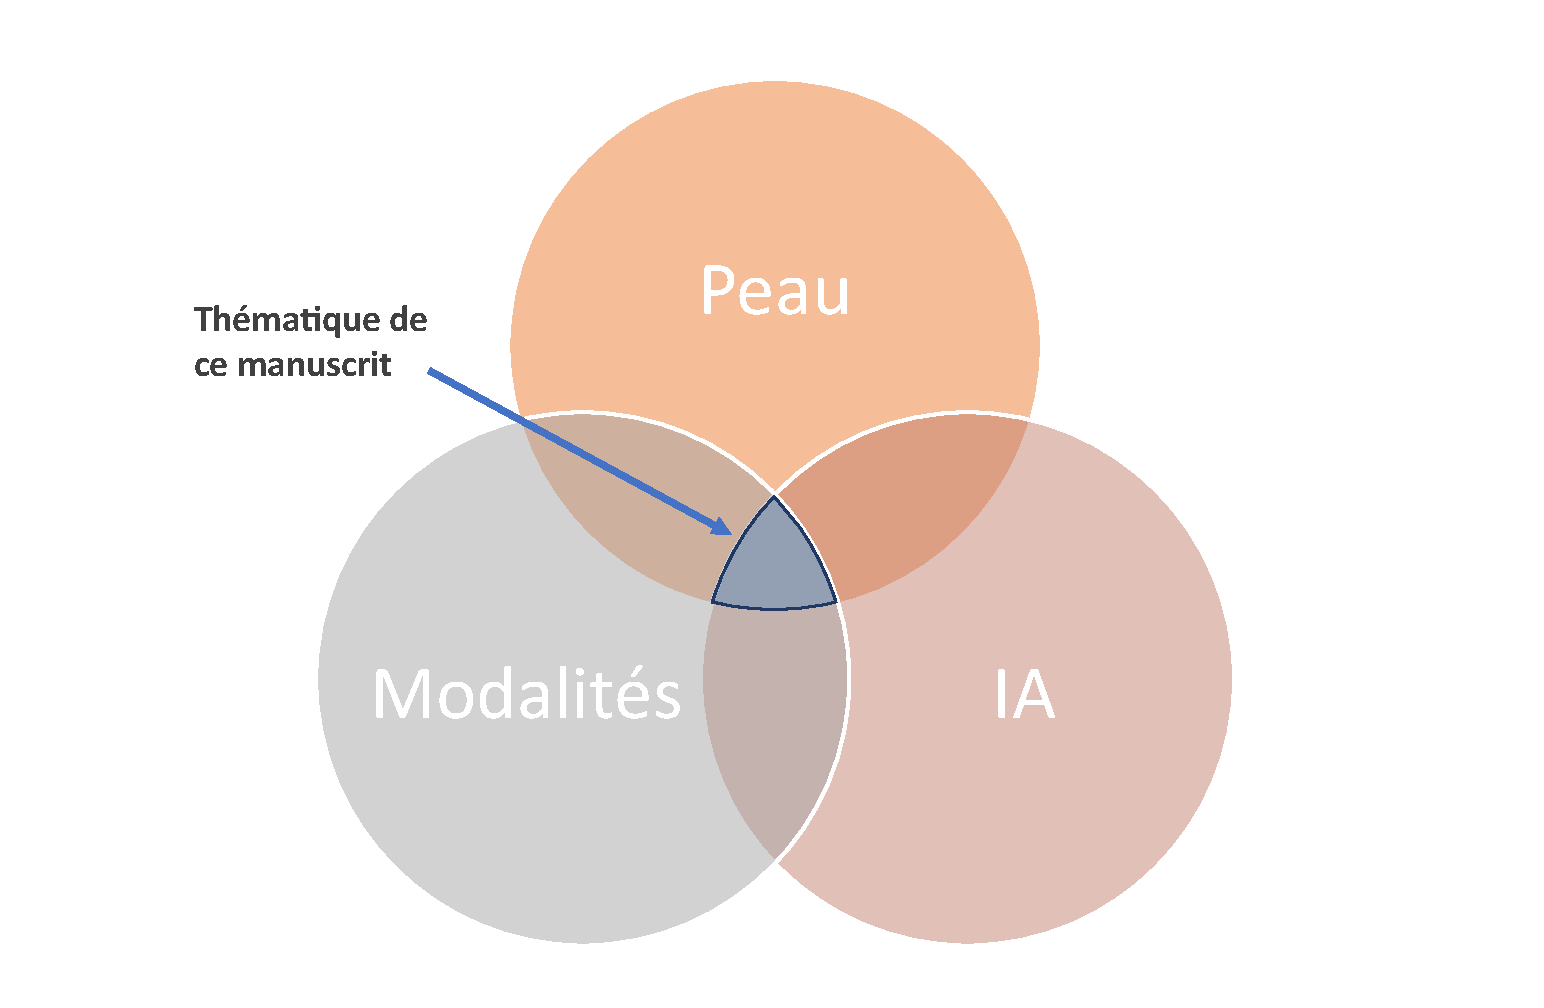
\includegraphics[width=0.8\linewidth]{contents/i_introduction/resources/scheme_our_work.pdf}
    \caption{Schéma de représentation des domaines impliqués de cette thématique de recherche. Notre travail se retrouve ainsi aux confluents de connaissances de la peau, des modalités d'imagerie permettant son acquisition et des domaines de l'intelligence artificielle.}
    \label{fig:scheme_our_work}
\end{figure}\par

Dans un premier temps, le contexte de cette étude est abordé dans la \Cref{part:contexte}. Cette partie débute par une présentation de la peau, l'organe majeur de cette étude, réalisée au sein du \Cref{chap:chapter_1}. Puis, s'ensuit une mise en évidence des principes d'interaction entre la peau et la lumière, avant de présenter les techniques de visualisation à la disposition des médecins dans le \Cref{chap:chapter_2}. Ensuite, le \Cref{chap:chapter_3} présente au lecteur l'ensemble des connaissances d'intelligence artificielle sollicitées dans ce manuscrit. Pour finir cette partie, le \Cref{chap:chapter_4} présente les données mise à disposition de cette étude mais également les principaux travaux en lien avec ce travail.\par

Dans un second temps, la prise en charge de la modalité \gls{rcm} est abordé par la \Cref{part:microscopy}. A cette fin, cette partie débute par le traitement des images de cette modalité dans le \Cref{chap:chapter_5} dédié à la classification de ces images et propose une extension de ces travaux dans le \Cref{chap:chapter_6}. Pour finir, le \Cref{chap:chapter_7} propose diverses méthodes permettant à partir des images de remonter à la prise de décision au niveau d'une lésion.\par

Dans un dernier temps, la finalité de ce travail est traitée par la \Cref{part:multimodal} dédiée à l'apport de l'information multimodale. Dans ce but, le \Cref{chap:chapter_8} reprend les conclusions de travaux sur les modalités d'imagerie clinique et de dermatoscopie ainsi que les conclusions issues de la précédente partie sur la modalité \gls{rcm} et propose des méthodes d'agrégation séquentielles de ces informations.\par